\documentclass{report}

% The ams packages are required to insert any mathematical symbols that you may require
\usepackage{amsfonts}
\usepackage{amssymb}
\usepackage{amsmath}
\usepackage{amsthm}
% This package is used for embedding things like PDFs and JPEGs into your document
\usepackage{graphicx}
% This package is used for drawing pictures (such as trees)
\usepackage{tikz}
\usetikzlibrary{arrows,automata}
% These packages are used for adding pseudo-code to your document
\usepackage{algorithm2e}
\usepackage{algorithmic}
% This package is for if you require an appendix
\usepackage{appendix}

\usepackage{datetime}
\usepackage{fancyhdr}
\usepackage{semantic}
\usepackage[noload]{qtree}
\usepackage{comment}
\usepackage{pdflscape}
\usepackage{graphicx}
\usepackage[margin=1in]{geometry}
\usepackage{moreverb}
\usepackage{caption}
\usepackage{url}
\usepackage{layout}
\usepackage{subfig}
\usepackage{lineno}

\linenumbers

\usepackage[annatar]{tengwarscript}

\usetikzlibrary{shapes}
\usetikzlibrary{arrows}

\newcommand{\pr}{\mathbb{P}}
\newcommand{\tengt}{\mbox{\Ttinco}}
%\newcommand{\tengt}{\Gamma}

\DeclareMathOperator*{\argmax}{arg\,max}
\DeclareMathOperator*{\argmin}{arg\,min}

\begin{document}

\begin{titlepage}
\title{An Investigation of Stochastic Processes on Human-Generated Data}
\author{Tim Jones}
%\maketitle

\centering{\textsc{\huge{An Investigation into Stochastic Processes for Modelling Human-Generated Data}}}\\[1.5cm]

\centering{\textsc{\large{A 20-cp 3rd year project}}}\\[1.5cm]

\begin{minipage}{0.4\textwidth}
\begin{flushleft} \large
\emph{Author:}\\
Tim Jones
\end{flushleft}
\end{minipage}
\begin{minipage}{0.4\textwidth}
\begin{flushright} \large
\emph{Supervisor:} \\
Dr. Gordon Ross
\end{flushright}
\end{minipage}\\[1.5cm]

\vfill

\begin{minipage}{0.4\textwidth}
Submitted: \dotfill
\end{minipage}

\vfill

Rendered on \today


\end{titlepage}

\tableofcontents

\chapter{Introduction}

Modelling human-generated ``random" data is notoriously difficult. In this project, we attempted to model the behavior of one user of twitter using various random processes. The user was observed over the course of around 6 months posting (emitting) a little over 3,300 tweets. The goal is to find some kind of model to fit these data, without using a hideously large number of parameters.

The data are visualised in Figure \ref{raw_data}. We see a little seasonality - the user seems to be going to sleep at some time, waking up at another time - but beyond that we'll be reliant on statistical tests to judge how good our model is.

\begin{figure}[h]
\includegraphics[width = \textwidth]{./images/raw_data.png}
\caption{The raw data gathered from the twitter user. Each blue cross marks a tweet at a particular time.}
\label{raw_data}
\end{figure}

\chapter{A Zoo of Stochastic Processes}\label{zoo}

\section{Markov Chains}

\subsection{A Formal Definition}

A stochastic process \cite[p590]{doob96} is a collection $\{X_t  | t \in T\}$ (sometimes $X(t)$ for continuous $T$) of random variables. These collections may be indexed arbitrarily, but tend to be used to describe the evolution of some random series of events, using $T$ to be some representation of either discrete or continuous time, for instance $X_t$ may be the number of observed emissions from a radioactive source after $t$ minutes or the lisence plate of the $t^{th}$ car to go past a speed camera.

A Markov Chain is a stochastic process with a particular property. We usually set $T=\{0,1,2,...\}=\mathbb{N}$ or $T =\{x | x \geqslant 0 \} = \mathbb{R}^{+}$. If $T=\mathbb{N}$ and each $X_t$ is a discrete random variable over the set $S$, then we say that $(X_t)_{t \in \mathbb{N}}$ obeys the Markov Property iff

$$
\forall t \in T, s \in S \quad \pr (X_{t+1} = s | X_0, X_1, ... X_t) = \pr (X_{t+1} = s | X_t)\cite{mwmarkov}
$$

Similarly, if $T=\mathbb{R}^{+}$, we have a continuous analogue to the Markov Property;

$$
\forall \delta > 0, s \in S \quad \pr (X(t+\delta) = s | \{X(\tau), \tau < t\}) = \pr (X(t+\delta) = s | X_t)
$$

If a stochastic process obeys the Markov Property, then we say that it is a Markov Chain. If a stochastic process obeys the continuous analogue to the Markov Property, then it is referred to as a Continuous Time Markov Process (CTMP). We refer to $S$ as the state-space, each $s \in S$ is a state, and $X_t$ represents the state at time t. We usually write the Markov Property as ``given the present, the future is conditionally independent of the past" \cite{mwmarkov}.
%COVER THIS IN G&S CITATIONS

We'll be dealing exclusively with discrete Markov Chains in this project, ie a Markov Chain where $S$ is discrete. In most cases, $S \subseteq \mathbb{Z}$, though our states can be integers, real numbers, popes, or any other completely arbitrary non-empty set. Where $S$ is discrete, we define $\mathbf{\delta} = (\delta_i)_{i \in S}$, the initial probability vector, and $\Pi = (\pi_{ij})_{(i,j) \in S^2}$, the matrix of transition probabilities, such that.
\begin{align*}
\delta_i &= \pr (X_0 = i) \\
\pi_{ij} &= \pr(X_{t+1} = j | X_t = i) \forall t \in \mathbb{N}
\end{align*}

Every discrete-state Markov Chain with $T=\mathbb{N}$ can be uniquley defined by the triple $(S,\delta,\Pi)$.

For CTMPs, we usually define the transition rate matrix $Q$ such that

$$
\forall i,j \in S, \delta>0 \quad \pr (X(t+\delta)=j|X(t)=i) = q_{ij}\delta + o(\delta)
$$

Where $o(\delta)$ is some function such that $o(\delta) -> 0$ as $\delta -> 0$. This gives us that

$$
\forall i,j \in S, \delta>0 \quad \pr (X(t+\delta)=j|X(t)=i) = (e^{\delta Q})_{ij}
$$

That is, the $i,j^{th}$ element of the matrix exponential of $\delta Q$. With the initial probability vector $\delta$ defined as before, we can uniquely define any CTMP with the triple $(S,\delta,Q)$.

\subsection{An Intuitive Interpretation}

Whilst the above defines Markovian Processes, it fails to describe them in any intuitive way. Before attempting to use them, it is important to be able to deal with both the continuous and discrete-time Markov Chains in an intuitive way. My personal preferred method is to use edge-weighted directed graphs\cite{mwgraph}. Each state in $S$ is given a node in the graph, and for each $i,j \in S$ the edge $(i,j)$ is given weight $\pi_{ij}$ in the discrete case and $q_{ij}$ in the continuous case.

As an example, let's use the following definitions, with $\delta$ and $\Pi$ indexed in the order the elements of $S$ are written;

\begin{align*}
S &= \{\mbox{John Paul II}, \mbox{Avian I}\}\\
\delta &= \left(1,0\right)\\
\Pi &=
\left(
\begin{matrix}
0.3&0.7\\
0.7&0.3
\end{matrix}
\right)
\end{align*}

This defines a Discrete Time Markov Chain with the following graph:

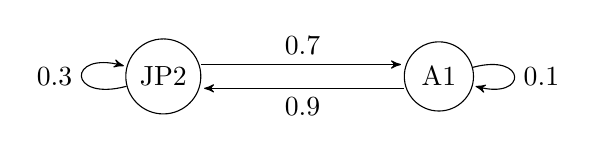
\begin{tikzpicture}[->,>=stealth',shorten >=1pt,auto,node distance=3.5cm]
  \node[state]         (r)                     {JP2};
  \node[state]         (b)  [right of = r]     {A1};

  \path  (r) edge[loop left]   node {$0.3$} (r)
         ([yshift=1ex]r.east) edge node {$0.7$} ([yshift=1ex]b.west)

         (b) edge[loop right]   node {$0.1$} (b)
         ([yshift=-1ex]b.west)edge node {$0.9$} ([yshift=-1ex]r.east)

  ;
\end{tikzpicture}

We can then say that a discrete Markov Chain will hop from node to node at each time step with probabilities defined by the weights of the edges between the current node and its neighbors. A CTMP is slightly more complex; on arriving in a state $i$, all neighboring states $j$ generate a random time $T_j ~ Exp(q_{ij})$. We let $k = \argmin_{j\in S} T_j$, and say that the CTMP will remain in state $i$ for $T_k$ units of time, then jump to state $k$.

\subsection{The Poisson Process}

The simplest form of CTMP is the homogeneous Poisson Process, where $S = \mathbb{N}$ and $\forall i \in S, q_{ii}=-\lambda, q_{i,i+1} = \lambda$. We call $\lambda$ the rate of this process. If N(t) is a Poisson process, we then have that

$$
\forall i \in \mathbb{N}, t,\delta \in \mathbb{R}^{+}, \pr (N(t+\delta) = i+1 | N(t) = i) = \lambda \delta + o(\delta)
$$

The graph for this process is similarly simple
%poot graph here

We can also sacrifice the Markov Property to define an inhomogeneous poisson process. Everything remains from before, except rather than having a rate parameter $\lambda \in \mathbb{R}^{+}$, we have a rate function $\lambda : \mathbb{R}^{+} -> \mathbb{R}^{+}$, where

$$
\forall i \in \mathbb{N}, t,\delta \in \mathbb{R}^{+}, \pr (N(t+\delta) = i+1 | N(t) = i) = \lambda(t) \delta + o(\delta)
$$

Since this process is no longer Markovian, it makes little sense to attempt to graph it, however it remains a powerful tool.

\section{Hidden Markov Models}

The Hidden Markov Model is an extention of the Markov Chain used for fitting various stochastic models.

With discrete time and state space, rather than having a directly observable Markov Chain, we assume that the process we observe has an underlying unobservable Markov Chain. We then define an observation space $O$, and a set of probability distrubtions, $\{p_s | s \in S\}$. Before jumping out of state $s$, the Markov Chain emits observation $o$ with probability $p_s(o)$. Alternatively, we can define a continuous $O$ with probability densities instead of a probability distribution.

The traditional example is that of the ``unfair casino". Imagine the dealer at the casino has two six-sided dice. Die one is fair, but die two is weighted such that it never shows a $6$, and shows the numbers 1 to 5 with equal probabilities. The dealer will clandestinely swap the dice with probability $0.1$ before rolling. Here, our state space is $\{1,2\}$ and our observation space is $\{1,2,3,4,5,6\}$. We can represent this as follows;
%POOT DIAGRAM HERE

We can only observe the results of the dice rolls, but what we're interested in is the underlying model. Firstly, we want to know what die the dealer is likely to be using at any given time - if I've seen the dealer roll a 6, I know he was using the fair die then, so he will use the fair die again with probability $0.9$, for example. Further to this, suppose we didn't know the above parameters in advance. We may also want to estimate them from observations in some way.

\chapter{Potential Modelling Techniques}\label{techniques}

For this project, we'll be modelling data generated by one of the most prevalent twitter users. The times of tweets were gathered over the course of 6 months, and stored in a file. The goal is to find a tight-fitting statistical model for it, without using an excess of parameters.

%Put pictures of data here

\section{Fitting a Non-Homogeneous Poisson Process}

The simplest place to start is with a non-homogeneous poisson process. We assume that the tweeter emits tweets according to a variable rate poisson process, and attempt to find its rate function. For convenience, we'll describe our time in hours, though naturally the units could be arbitrary. We start by simulating a poisson process of known rate, and seeing how well we can recover the original rate function. We start with a simple step function,

$$
\lambda(t) = 
\begin{cases}
5  \mbox{for} 0  \leqslant t < 30\\
10 \mbox{for} 30 \leqslant t < 50\\
5  \mbox{for} 50 \leqslant t < 100
\end{cases}
$$

And we simulate the process for 100 hours, producing a trace such as;

%Put trace here

We can fit a step function by taking the differences in emission times, then attempting to cluster them. The results from this seem to fit the rate function fairly well

%Diagram here

But if we try something more complex, eg $\lambda(t) = 5+5sin(t)$, we have some issues. This is a very high-rate process which generates a lot of data with each trace. With 100 traces, giving us roughly 3,000 data points, our clustering starts to fail after just 4 rates.

We could instead attempt to fit a polynomial function, but a smooth function is subject to one very large problem with twitter data. Humans don't behave in a smooth manner. Our usage of twitter throughout a day does not vary along some continuum, and has some odd properties. See the following trace of a single day;

% Trace of one day, showing bursts

We can see an important feature between 
%time1
and
%time2
. We'll call this a ``burst". The user is tweeting very rapidly for a short period of time. These bursts occur at random times throughout the day, and last for random lengths of time, but they all take on the same form. This heavily restricts our function. We can't simply say that at some particular time there is always a burst, but we also cannot deny their existence by smoothing them out since these bursts, by their very nature, will account for the majority of the observed tweets.

Clearly, a different approach is needed.

\section{Fitting a Markov-Modulated Poisson Process}

The Markov-Modulated Poisson Process (MMPP) is a particularly devious form of Hidden Markov Model. We assume that, underlying the tweeter, there is a CTMP. Each state is tied to a fixed Poisson Process rate. Whilst the process is in a particular state, it emits observable emissions according to a poisson process of that rate. We can simulate one of these with the following algorithm;

%MMPP Simulation algorithm goes here

Such a model seems ideal, capturing the simplicity of a step function, and letting us model the idea of randomly distributed bursts throughout a day. Indeed, several authors have postulated that such a model would be ideal for simulating human behavior %lots of citations go here
but there have so far been no actual quantifiable studies of its relevance. Part of the reason for this is likely the lack of algorithms.

Fitting a Hiddin Markov Model of any kind relies on two main algorithms, Baum-Welch %cite
and Viterbi
%cite
. The Baum-Welch Algorithm is an expectation-maximisation algorithm for finding the transition probabilities/rates and the emission probabilities, given a set of possible emissions, a number of states to fit and an observed sequence of emissions. Viterbi will take an observed sequence of emissions and the parameters of an HMM, and produce the most likely state in which each of these emissions happened. The HiddenMarkov package hosted on CRAN %cite
is the only easily-accessible Hidden Markov Model package which supports the Markov Modulated Poisson Process, but does not contain any implementation of the Viterbi algorithm. It therefore became necessary to write one.

\subsection{A derivation of the classical viterbi algorithm}

The Viterbi algorithm for a standard Discrete Time Hidden Markov Model relies on a known, finite observation space $O$, a known distribution on $O$ for each state $s$, $p_s$, and known transition probabilities $\pi_i,j$, with known initial probabilities for each state $s$, $\delta_s$. We let $[k] = \{1,2,...,k\}$. The goal is, given a sequence of T observations $(y_n)_{n \in [T]}$, $y_i \in O$, to find the sequence of states $(x_n)_{n \in [T]}$ satisfying

$$
\mathbf{x} = \argmax_{\widehat{\mathbf{x}} \in S^T} \pr(\mathbf{\widehat{x}} | \mathbf{y})
$$

We call $\mathbf{x}$ the Viterbi Path.

We let $V_{t,s}$ be the probability of the most probable state sequence responsible for the first $t$ observations which ends in state $s$ %cite http://www.cs.cmu.edu/~epxing/Class/10701/Lecture/lecture12-HMM.pdf
. We have that $V_{1,s}$ is the probability of both being in state $s$ at time 1 and seeing observation $y_1$ from state $s$. A simple application of Bayes' Rule gives us that

$$
V_{1,s} = \pr (y_1|s)\pr(x_1=s)
$$

Recall that $\delta_s$ is the probability of being in state $s$ at time 1, ie $\pr(x_1=s)$, and that $p_s(y_1)$ is the probability of observing $y_1$ from state $s$, ie $\pr (y_1|s)$. Both of these parameters are estimated by the Baum-Welch algorithm, hence,

$$
V_{1,s} = p_s(y_1)\delta_s
$$

Given $V_{\tau,s}$ for $\tau < t$, we can find $V_{t,s}$ by noting that the Markov Property implies a form of memorylessness. Given the present, the future is conditionally independent of the past. As such, we need only consider $V_{t-1,s}$ for each $s$, as well as our known parameters. 

The probability of the most likely path that leads us to state $s$ at time $t$ is given by the probability of the most likely path that led us to $s'$ at time $t-1$, and then jumped to $s$ at time $t$, and then emitted $y_t$ from state $s$. The probability of jumping from $s'$ to $s$ is $\pi_{s',s}$. The probability of emitting $y_t$ from state $s$ is $p_s(y_t)$. The probability of the most likely path that leads us to $s'$ at time $t-1$ is $V_{t-1,s'}$. Hence,

$$
V_{t,s} = p_s(y_t) \max_{s'\in S} (\pi_{s',s}V_{t-1,s'})
$$

Using this recurrence, we can find $V_{t,s} \forall t \in [T]$ by a standard dynamic programming algorithm.

From here, we can then work backwards to find the Viterbi path. $x_T = \argmax_{s \in S} V_{s,t}$ - the most likely final state is the state in which the path of maximum probability ends.

Let
 
$$
T_{s,t} = \argmax_{s'\in S}(\pi_{s',s}V_{t-1,s'})
$$

Ie, $T_{s,t}$ is the state from which we are most likely to have come at time $t-1$ given that we are in state $s$ at time $t$, we can then see that $x_{t-1} = T{x_t,t}$. Note the similarities in the definitions of $V$ and $T$ - both can be calculated simultaneously - $V$ is the maximum, $T$ is the argument that maximises. $T_{s,1}$ is never used, so need never be defined. 

Since we have an expression for $x_{t-1}$ in terms of $x_t$, and for $x_T$, we can then recover $\mathbf{x}$, the Viterbi Path. We can therefore define the viterbi algorithm as follows:

%Put algorithm here

\subsection{A First Approximation of the Viterbi Algorithm for the Markov-Modulated Poisson Process}

Recall the dependencies for the DTHMM Viterbi Algorithm. We require knowledge of a finite $O$, $p_s$ for each $s$, and $\pi_{ij}$ for each pair of states $i,j$.

In an MMPP, we observe a Poisson Process of rate randomly varying between various known rates - the rates being our states. Let $S = \{\lambda_1,...,\lambda_m\}$. Our observations can be interpreted as exponential random variables of these rates. Let $\tau_0 = 0$, and $\tau_i$ be the time of the $i^{th}$ poisson emission for $i \in [n]$. Let $y_i = \tau_i-\tau_{i-1}$ for $i \in [n]$. Given that the underlying CTMP was in state $\lambda_s$ at time $\tau_i$, we have that $y_i \sim Exp (\lambda_s)$. From the properties of the generic CTMP, the probability that the process is in state $j$ at time $\tau_i$ given that it was in state $i$ at time $\tau_{i-1}$ is given by $(e^{Qy_i})_{\lambda_{i},\lambda_{j}}$. To ease notation, we'll write this as $(e^{Qy_i})_{i,j}$, omitting the $\lambda$s.

The state space $S$ and transition rates $Q$ are estimated by the Baum Welch algorithm as before, so after running Baum Welch over an observed trace, we can start to find the most likey state at each emission. Note that this ``Viterbi Path" is not the most likely sequence of state transitions, it is instead the most likely state in which the underlying CTMP resides at the time of each emission. This quirk is discussed in %APPENDIX REF

Since our emissions are continuous, we don't have any notion of ``most probable" - if we model height continuously, the probability that I meet someone exactly 1.8m tall is the same as the probability that I meet someone exactly 18m tall, they're both 0 - so instead we'll base our likelihood calculations off probability density - capturing the idea that, even though I don't know for certain that I'll meet one of the two, it's more likely for me to meet the 1.8m tall person.

We let $p_s(t)= \lambda_s e^{-t\lambda_s}$, the probability density of an exponential random varaible of rate $\lambda_s$ evaluated at $t$. Let $V_{t,s}$ be the probability density of the most likely path that leads us to emitting $y_t$ from state $s$. We have that

$$
V_{1,s} =  \delta_{s}p_s(y_1)
$$

The probability density of the most likely path that leads us to waiting for time $y_1$ before making an emission is given by the probability of starting in state $s$, multiplied by the probability density of waiting $y_1$ for an emission from state $s$. The memorylessness property of a CTMP allows us to only consider $V_{t-1,s}$ when calculating $V_{t,s}$. We have that

$$
V_{t,s} = p_s(y_t) \max_{s'\in S} (V_{t-1,s'}(e^{Qy_t})_{s',s})
$$

The probability density of the most likely path that leads us to waiting for time $y_t$ between the $(t-1)^{th}$ and $t^{th}$ emissions in state $s$ is given by the probability density of the most likely path that takes us to state $s'$ for the $(t-1)^{th}$ emission, followed by jumping (along any arbitrary path) into state $s$ for emission $t$, multiplied by the probability density of emitting $y_t$ in state $s$.

From here, we can proceed as normal. We define $T$ as before to record our most likely states at each transition, and work backwards to find $\mathbf{x}$, producing the following algorithm

%ALGORITHM GOES HERE

The reason that this is an approximation is the fact that the algorithm assumes that either a jump happens instantaneously, or not at all - we always evaluate $p_s(y_t)$, rather than $p_s(y_t-\tengt)$\footnote{\tengt - tinco - represents the voiceless alveolar stop in the Tengwar alphabet, as devised by JRR Tolkein. When dealing with time so frequently, we eventually run out of ways to write the letter t}, where $\tengt$ represents the time we wait for all the relevant transitions to occur. The times between state transitions are exponentially distributed, and we are dealing with the most likely outcomes. The most likely outcome of any exponential distribution is $0$ so, if the underlying CTMP jumps from one state to another, the most likely time for that jump to happen is immediately, so $\tengt = 0$. If multiple jumps happen, their individual times are exponentially distributed, but their sum does not have a mode of 0.

This first approximation is in fact very powerful. Approximating in this way assumes that multiple transitions between emissions are rare, alternatively  that emissions within each state are more frequent than transitions out of that state. If the converse is true - transitions out of the state are more frequent than emissions within the state - then we have an odd situation whereby some state is frequently entered and then left again with no emissions happening. Whilst such states are perfectly valid and can indeed exist in a theoretical MMPP, detecting one in reality with no prior knowledge is very difficult.

As a final note, we can further refine the fitted model based on the results of the Viterbi algorithm by changing the estimated rate of each state to the observed rate of the emissions estimated to occur in that state. By the nature of these estimation algorithms, these results are likely to differ, and with a large sample size what we observe is usually closer to the truth than what we assert.

\subsection{Applying the Algorithm}

The algorithm was written in R and added to the pre-existing HiddenMarkov %cite
package as acquired from The University of Bristol's CRAN Mirror, which was then recompiled to be loaded into an R environment. A Python script was written to call into this library from a more conveneint language using RPy2%cite
, with mathematical, statistical and visualisation functions loaded from PyLab%cite
. The data was preprocessed such that rather than recording exact times and dates of tweets, it instead recorded time since the beginning of the observation in hours at which each tweet occured. This was then fed into a HiddenMarkov MMPP, over which BaumWelch and Viterbi were then run based on the assumption of 3 states. The resulting model was as follows:

%LOTS OF MODEL STUFF GOES HERE

And, with the states shaded in in the colours represented above, the transitions were as follows:

%Big pile of diagrams

From this distance, we already see at least some kind of sensible behavior - the user seems to have regular sleeping patterns, tweeting during the day and not tweeting at night-time. Zooming in on a single day, we see some more sensible results - the burst mentioned before has been noticed and highlighted, and the normal day-to-day tweets all remain in the same state.

We can evaluate this model by performing a Kolmogorov-Smirnov test on the data for each state. It should follow an exponential distribution. Running this test, we find, however, that it very much does not;

% KS results here

Whilst 3 states makes sense intuitively, there's no reason why this is definitely the case, so let's try different numbers of states. We can find the most optimal number based on the Bayesian Information Criterion %cite and define
. 500 iterations of BaumWelch were run over the data until a local obtimum was reached. This optimum occured at 7 states, described as follows:

%More model stuff

Fitted by the same methods, we see the following results

%Diagram-tastic

Unfortunately, the Kolmogorov-Smirnov tests still fail. Fitting more states would probably give a better fit, but due to the quadratic scaling it would also start sending the number of parameters up to absurd levels.

\subsection{An Alternative Approach}

From this point, it is starting to seem like the tweeter does not follow an MMPP, but there is one last thing we can attempt in this vein. A DTHMM can still have a continuous observation space and all the previous methods will work, just with probability density in place of probability. Rather than observing a series of times, we will instead observe a series of time differences, and look for any small number of states that lets us gather these differences into the same exponential distribution. The results from such a model will be similar, but lose some information about how long our tweeter actually spends in each state. The crucial difference between the two is that in an MMPP emissions and transitions take place along the same timeline - compare the Viterbi algorithms for both the MMPP and DTHMM, and note that the transition probabilities between a DTHMM's states do not depend on the observed emissions, whilst the transition probabilities in the MMPP version do.

So we go through the same procedure again - start by fitting the intuitive 3 states to find the following model;

% Stuff goes here

Then use the Bayesian Information Criterion to note that the optimal number of states is, again, 7;

% More stuff here

And finally perform some new KS tests to find that...

%Results of KS test

The data cannot be well-clustered into a small number of exponentially distributed subsets. We can then conclude that these data do not follow any kind of simple poisson process, in spite of appearances.

\section{A Zoo of Problems}

\section{The Markov-Modulated Generalised Time Process}

\appendix
\chapter{Fun with Integrals}\label{fun}

Recall Figure \ref{trace_nonhom1}. It is a trace of an inhomogeneous Poisson process with the following rate

$$
\lambda(t) = 
\begin{cases}
5  & \mbox{for} \quad 0  \leqslant t < 30\\
10 & \mbox{for} \quad 30 \leqslant t < 50\\
5  & \mbox{for} \quad 50 \leqslant t < 100
\end{cases}
$$

Figure \ref{integral_fun_1} shows a Poisson process of rate $\lambda$, alongside the integral of $\lambda$. With only 600 samples, the two functions seem similar. Let $N$ be an inhomogeneous Poisson process of rate $\lambda: \mathbb{R}^{+}->\mathbb{R}^{+}$, let $\delta > 0$, and consider the following;

\begin{align*}
\pr (N(t+\delta)-N(t) = 1) &= \lambda(t)\delta + o(\delta)\\
\pr (N(t+\delta)-N(t) > 1) &= o(\delta)\\
\mathbb{E}[N(t+\delta)-N(t)] &= \sum_{i=1}^\infty \pr (N(t+\delta)-N(t) = i)\\
&= \lambda(t)\delta + o(\delta)\\
\\
\lim_{\delta->0} \frac{\mathbb{E}[N(t+\delta)-N(t)]}{\delta} &= \lim_{\delta->0} \frac{\lambda(t)\delta + o(\delta)}{\delta}\\
&= \lambda(t)
\end{align*}

So if $N$ is a Poisson process of rate $\lambda$, then it's also a function whose value we expect to increase at a rate of $\lambda$ meaning that, with enough samples, $N$ would approximate an indefinite integral of the function $\lambda$. Currently, the standard method for evaluating difficult integrals computationally is to use the Monte-Carlo ``dartboard" algorithm \cite[\textsection 2]{montecarlo}, though this is only capable of evaluating a single, definite integral. If we had an approximation of the indefinite integral function, we could evaluate arbitrarily many definite integrals by just looking up values from the function. Figure \ref{integral_fun_2} shows an aproximation of the integral of $\sin\left(\frac{x}{5}\right)+1$, taken by simulating 50 Poisson process for a total of roughly 5,000 emissions, each emission only incrementing the process by $0.02$, rather than 1. Here, we see a very close approximation of the true integral. The dartboard algorithm usually uses tens of thousands of randomly generated points to evaluate a single definite integral.

\begin{figure}[h]
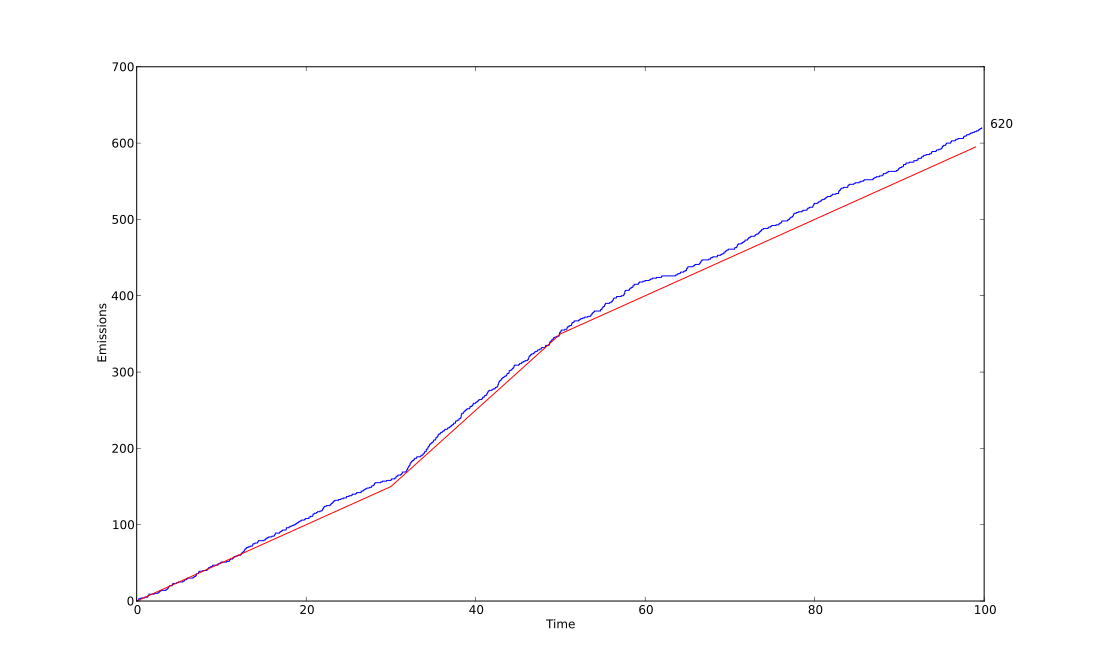
\includegraphics[width = \textwidth]{./images/integral_fun_1.png}
\caption{A trace of an inhomogeneous Poisson process used to estimate an integral, alongside its true integral, plotted with 620 Poisson emissions}
\label{integral_fun_1}
\end{figure}

\begin{figure}[h]
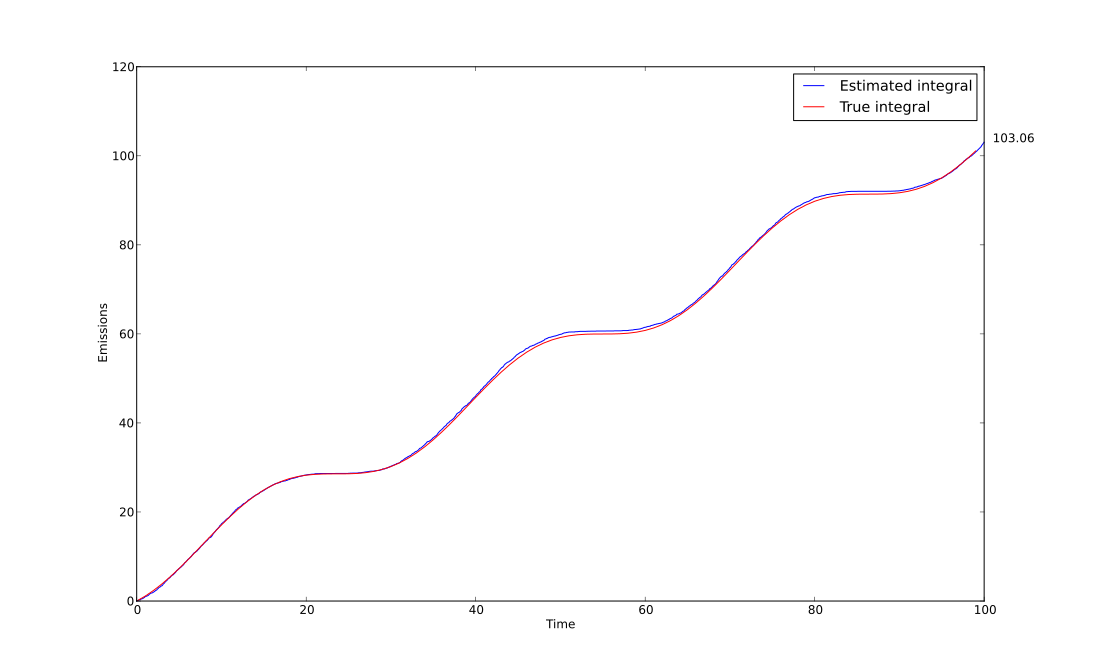
\includegraphics[width = \textwidth]{./images/integral_fun_2.png}
\caption{A trace of an inhomogeneous Poisson process used to estimate an integral, alongside its true integral, plotted with 5153 Poisson emissions}
\label{integral_fun_2}
\end{figure}

Of course, the actual practicalities of such an algorithm and its relevance to higher-order integrals are yet to be confirmed, though it could be an interesting area for further study.

\begin{thebibliography}{9}

\bibitem{mmpp1} Ihler,A.,Hutchins,J.,\& Smyth,P Learning to detect events with Markov-Modulated Poisson Processes.

ACM Transactions on Knowledge Discovery from Data, 1(3), 13. 2007 

\url{http://dl.acm.org/citation.cfm?doid=1297332.1297337}

\bibitem{mmpp2} R.D. Malmgren, D.B. Stouffer, A.E. Motter, and L.A.N. Amaral, A Poissonian explanation for heavy tails in e-mail communication, 

PNAS, 105(47):18153–18158, 2008 

\url{http://www.pnas.org/content/105/47/18153}

\bibitem{mmpp3} Scott, S. L. and Smyth, P. 2003. The Markov modulated Poisson process and Markov Poisson cascade with applications to web traffic data.

Bayesian Statistics 7, 671–680. 

\url{http://dl.acm.org/citation.cfm?doid=1297332.1297337}

\bibitem{doob96}
	Joseph L. Doob, The Development of Rigor in Mathematical Probability (1900-1950)

	The American Mathematical Monthly, Vol. 103, No. 7 (Aug. - Sep., 1996), pp. 586-595

	\url{http://www.jstor.org/stable/2974673}

\bibitem{mwmarkov}
	Weisstein, Eric W. ``Markov Chain." From MathWorld--A Wolfram Web Resource. 

	\url{http://mathworld.wolfram.com/MarkovChain.html}

\bibitem{mwgraph}
	Weisstein, Eric W. ``Graph." From MathWorld--A Wolfram Web Resource. 
	
	\url{http://mathworld.wolfram.com/Graph.html}

\bibitem{thinning}
	Lewis, P. A. W. and Shedler, G. S. (1979), Simulation of nonhomogeneous Poisson processes by thinning.

	Naval Research Logistics, 26: 403–413.

	\url{http://onlinelibrary.wiley.com/doi/10.1002/nav.3800260304/abstract}

\bibitem{hiddenmarkov}
	David Harte. \emph{HiddenMarkov} v1.7-0, a Hidden Markov Model library written in R and Fortran, 

	\url{http://cran.r-project.org/web/packages/HiddenMarkov/index.html}

\bibitem{matplotlib}
	Hunter, J. D. \emph{MatPlotLib}, a 2D graphics environment 

	\url{http://matplotlib.org/}

	IEEE Computer Soc, Vol. 9, No. 3 (2007), pp. 90-95

\bibitem{gimpdiff} The GIMP Development Team. \emph{The GIMP docs}, the documentation for the GNU Image Manipulation Program, 

\url{http://docs.gimp.org/en/gimp-concepts-layer-modes.html}

\bibitem{gimpthresh} The GIMP Development Team. \emph{The GIMP docs}, the documentation for the GNU Image Manipulation Program, 

\url{http://docs.gimp.org/en/gimp-tool-threshold.html}

\bibitem{rpy} Moriera W, Warnes GR, Gautier L. \emph{RPy} v2-2.3, a Python to R interface

\url{http://rpy.sourceforge.net/}

\bibitem{scipy} Jones E, Oliphant T, Peterson P \& others, \emph{SciPy}, open source scientific tools for Python, 2001-

\url{http://www.scipy.org}

\bibitem{baumwelch} Baum L.E, Petrie T, Soules G, \& Weiss N, A maximization technique occuring in the statistical analysis of probabilistic functions of Markov chains.

Annals of Mathematical Statistics 41(1), 164-171, 1970

\url{http://projecteuclid.org/DPubS?service=UI&version=1.0&verb=Display&handle=euclid.aoms/1177697196}

\bibitem{viterbi} Forney G.D, Jr., ``The viterbi algorithm,"

Proceedings of the IEEE , vol.61, no.3, pp.268,278, March 1973

\url{http://ieeexplore.ieee.org/stamp/stamp.jsp?tp=&arnumber=1450960&isnumber=31166}

\bibitem{bic} Schwarz, G. (1978) "Estimating the Dimension of a Model"

Annals of Statistics, 6, 461-464.

\url{http://projecteuclid.org/DPubS?service=UI&version=1.0&verb=Display&handle=euclid.aos/1176344136}

\bibitem{kmeans} Jones E, Oliphant T, Peterson P \& others, \emph{SciPy}'s k-means algorithm, \url{http://docs.scipy.org/doc/scipy/reference/cluster.vq.html}

\bibitem{mwlognormal} Weisstein, Eric W. "Log Normal Distribution." From MathWorld--A Wolfram Web Resource.

\url{http://mathworld.wolfram.com/LogNormalDistribution.html}

\bibitem{montecarlo} Caflisch E, Monte Carlo and quasi-Monte Carlo methods,

Acta Numerica vol. 7, Cambridge University Press, 1998, pp. 1–49.

\url{http://websrv.cs.fsu.edu/~mascagni/Caflisch_1998_Acta_Numerica.pdf}

\end{thebibliography}

\end{document}
